\section{Fast Hydraulic Erosion Simulation and Visualisation on GPU}
The behaviour of water massively influences the look and features of a terrain. Depending on the timespawn, amount of water, ground composition and many more factors, hydraulic erosion creates a variety of different, but distinctive ground deformations, such as ripples, ridges, meanders, riverruns and valleys. 
This paper \cite{Neidhold:2005:IPB:2381356.2381361} presents an approach capable of creating such deformations in short amount of time, making it suitable for interactive visualization. The model represents terrain and water surfaces using heightfield, which is sampled onto a regular grid. A shallow water model is used to update the water surfaces and the fluid velocity field. 

\subsection{Water simulation}
This paper uses a simplified Navier-Stokes equation to simulate the water flow. The approach discards 3D-features like mutiple water layers, vertical vortices and waves. this makes the equation less physically correct, but much faster to compute. The appraoch is based on a system of first order differential equations. This system describes the movement of material, in this case the amount of water at each cell, depending on velocity $\vec{v}$ and acceleration $\vec{a}$. Since this approach is dealing with complex erosion, the system uses am multidimensional material vector storing additional parameters like dissolved sediment.
$$\dot{\vec{v}} = \vec{a} -K_A \cdot \vec{v}=\frac{\vec{F}}{m} - K_A\cdot \vec{v}$$
$$K_A$$ describes the friction between the fluid and the terrain and can be manipulated for test purposes. 

A vector field assumes that the particles movement is constant. In a common Newtonian Physic System objects are accerlated by the gravity. The direction of acceleration is the direction of the biggest tile angle $\alpha$ of the underlying height field. Therefore the acceleration force can be computed from the sinus of $\alpha$ times the gravitational constant g. The angle $\alpha$ is determined by the gradient $\nabla I(x,y)$ of the height field. 

At this point he acceleration direction is only defined in x and y direction. The acceleration vector $\vec{M}$ can be computed using the gradient $\nabla I(x,y)$: 
$$\vec{M} = (- \frac{\Delta I}{\Delta x}, - \frac{\Delta I}{\Delta y}, - \frac{\Delta I^2}{\Delta x^2}, - \frac{\Delta I^2}{\Delta y^2})^T$$
The acceleration vector can now be computed as follow: 
$$\vec{a}= \frac{|\vec{M}_z|}{|\vec{M}|} \cdot g \cdot \frac{\vec{M}}{|\vec{M}|}$$

$\vec{M}_z$ describes the acceleration direction direction along the z axis.

\begin{figure}[htb]
	\centering
	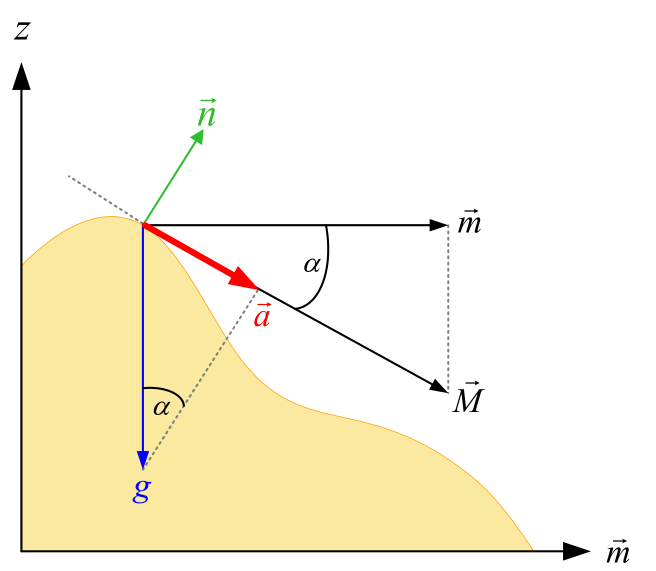
\includegraphics[width=.8\linewidth]{NWD05/acceleration}
	\caption{Calculation of acceleration.}
	\label{fig:calc_acceleration}
\end{figure}

\subsection{Hydraulic erosion function}
When water flows, soil, stones and other materials are dislocated and transported to lower regions. To simulate this effect the paper defines a hydraulic erosion function. Whenever a part of a material is moved to another grid cell by the simulation, this function is used. It determines the amount of disolved and deposited parts of material. 